\documentclass{article}
\usepackage[table]{xcolor}
\usepackage{float}
\usepackage{array}
\usepackage{graphicx}
\usepackage[spanish, es-tabla]{babel}
\usepackage[utf8]{inputenc}
\usepackage{csquotes}
\usepackage[margin=1.55cm]{geometry}
\usepackage{wallpaper}
\usepackage[depth=3]{bookmark}
\usepackage[
backend=biber,
style=numeric,
]{biblatex}
\addbibresource{references.bib} 
\setlength{\parskip}{1em}
\parindent 0px

\newcolumntype{P}[1]{>{\centering\arraybackslash}p{#1}}
\newcolumntype{M}[1]{>{\centering\arraybackslash}m{#1}}
 

\newcommand\signature{
\noindent\begin{minipage}{10cm}
    \noindent\vspace{3pt}\par
    Firma: \rule{7cm}{1pt}
    \noindent\vspace{15pt}\par
\end{minipage}}

\begin{document}

\begin{titlepage}


    \ThisLRCornerWallPaper{1}{imgs/fondo_tt.png} % Fondo de portada 
        \begin{center}
            \LARGE \textbf{Instituto Politécnico Nacional}\\*[0.3cm]
            \Large \textbf{Escuela Superior de Cómputo}\\
            \vspace{1cm}
            \rule{12cm}{0.5mm}\\*[0.3cm]% Línea {Longitud}{Grosor}
            \hspace{0.9cm} 
            %\normalsize {\textit{Ingeniería en Sistemas Computacionales}}\\
            %%%%  TITULO Y NÚMERO DE TRABAJO   %%%%
    		\LARGE \textbf{ Aplicación móvil gamificada de aritmética\\}
    		\LARGE \textbf {\emph{Trabajo Terminal No }} 
    		\vspace{1cm} %Espacio vertical
    	\LARGE \textbf{\\ Ingeniería en Sistemas Computacionales\\}
    	Alumnos: *Pineda Vieyra Itzcoatl Rodrigo, Mothelet Delgado Izaird Alexander\\
	Directores: Elena Fabiola Ruiz Ledesma, Lorena Chavarría Baez\\
	e-mail: itzcoatlpv@gmail.com
    \vspace{1cm} %Espacio vertical
        \end{center}

    \centering %Todo centrado
    \vspace{1cm} %Espacio vertical

    %%%%   ALUMNOS   %%%%
   	


\end{titlepage}

\tableofcontents
\pagebreak
\section{Introducción}
La intervención educativa requiere de una previa comprensión de la adquisición y desarrollo de la competencia aritmética
que está en la base de todas las posteriores dificultades y trastornos del aprendizaje matemático. Hay dificultades que
pueden surgir a lo largo de este proceso(desde nivel básico), lo que repercute en la resolución de ejercicios y problemas matemáticos avanzados.
Por lo que el desarrollo de la destreza operatoria aritmética es fundamental para que el estudiante, tanto de nivel básico como medio superior, pueda enfrentar con
éxito situaciones más complejas en el campo de la Matemática. Además, se requiere motivar al estudiante al desarrollar
trabajo operatorio aritmético, ya que en ocasiones su desarrollo puede resultar monótono y aburrido. Para ayudar al desarrollo de la destreza operatoria de los estudiantes se propone una aplicación gamificada móvil que promueva la
resolución de ejercicios aritméticos.

\subsection{Motivación}
La Aritmética como la Geometría son de las disciplinas matemáticas más antiguas y necesarias en la historia del género humano \cite{coronado2014estudio}. 
Su utilización funcional es requerida para las personas que participamos de esta sociedad, como medio de comunicación y comprensión de multitud de fenómenos que nos rodean, es por ello que el desarrollo de la destreza operatoria aritmética es una de las habilidades más necesitadas en la alfabetización socio instrumental.
Los niveles de fracaso en el aprendizaje matemático son preocupantes, especialmente en los últimos cursos de escolaridad obligatoria (secundaria). Los resultados de estudios internacionales como el Programa Internacional para la Evaluación de Alumnos de la OCDE (PISA)\cite{oecd2014what,oecd2016low} muestran que el aprendizaje matemático es el que presenta mayor porcentaje de fracaso \cite{coronado2016academic, mullis2016timss}. El cálculo es un componente esencial en la resolución de problemas aritméticos, y éste es uno de los contenidos más importantes de las matemáticas, junto a la geometría, la medida o la probabilidad. 
Es por ello que un elevado porcentaje de las dificultades de aprendizaje de las matemáticas tiene un origen aritmético, donde el cálculo representa un papel esencial \cite{orrantia2006dificultades}. Las habilidades numéricas y aritméticas son predictores críticos del futuro éxito o fracaso académico matemático\cite{rodriguez2017marcadores}. 

Se ha observado en declive las habilidades operatorias aritméticas de estudiantes 
universitarios\cite{tariq2002decline,carpenter2017psychology,huang2013gamification}. 
El estudiante cree que podrá contar con la calculadora de su celular en todo momento, 
pero cuando esto no se le permite, como en los exámenes de admisión, la falta del 
entrenamiento del cálculo mental entorpece la solución correcta de los reactivos 
de dichos exámenes. Por otra parte, el no fortalecer la destreza operatoria, afecta 
diferentes procesos cognitivos al llegar a la edad adulta\cite{martin2003loss}.
El presentar al estudiante los ejercicios de una forma rutinaria muchas veces provoca 
aburrimiento y desmotivación. 
También es fundamental la motivación y el estado emocional de los estudiantes en su desempeño académico. La motivación y estado emocional de los estudiantes es un factor clave en su desempeño académico\cite{larrazolo2013habilidades,ryan1997should}. Si deseamos que los jóvenes 
mexicanos tengan un mejor desempeño en el área de las Matemáticas, se requiere presentarles 
distintas formas de aprender y practicar sus conocimientos. Para ello una estrategia de 
apoyo es la gamificación, la cual se empleará para incentivar a los estudiantes de educación 
media superior a desarrollar su destreza operatoria.

\subsection{Plantamiento del Problema}
La problemática que se pretende atacar es la necesidad de fortalecer la destreza operatoria aritmética de los estudiantes de nivel básico y  medio superior [13], [14], lo cual es importante para el desarrollo del pensamiento matemático de los estudiantes. 
\subsection{Objetivos}
\subsubsection{Objetivo General}Desarrollar una aplicación móvil que apoye al estudiante de nivel básico y  medio superior en la 
adquisición de habilidades y conocimientos elementales, para fortalecer la destreza 
operatoria en  Aritmética, con el uso de la gamificación.

\subsubsection{Objetivos Específicos}
\begin{itemize}
	\item Diseñar actividades gamificadas, empleando números enteros con las 4 operaciones básicas.
	\item Desarrollar un módulo evaluador expresiones.
	\item Desarrollar un módulo de logros y mecánicas.
	\item Validar la aplicación móvil. 
\end{itemize}
\subsection{Estado del Arte}
\begin{table}[H]
\centering
\begin{tabular}{|c|M{6cm}|M{5cm}|}
\hline
Software & Características & Precio en el mercado \\ \hline

Fraction Challange & 
\begin{itemize}
	\item PVP local
	\item rondas con tiempos
\end{itemize} & 
Gratuito con micro transacciones \\ \hline


1+2=3 & 
\begin{itemize}
	\item Sumas y restas de enteros
	\item Tablas de liderato 
\end{itemize}& 
Gratuito \\ \hline


Fracciones calculadora & 
\begin{itemize}
	\item Calculadora de fracciones
\end{itemize}& 
Gratuito \\ \hline


Math Games & 
\begin{itemize}
	\item Logros
	\item Tablas de liderato
	\item Estadísticas
	\item Tutoriales de como realizar operaciones básicas
\end{itemize} & 
Gratuito con contenido bloqueado(se puede desbloquear haciendo un pago único) \\ \hline

Arithmetic Practice & 
\begin{itemize}
	\item Logros
	\item Tablas de liderato
\end{itemize} & 
Gratuito con contenido bloqueado(se puede desbloquear haciendo un pago único) \\ \hline


Mental Arithmetic  & 
\begin{itemize}
	\item PVP local
	\item Logros
	\item Tablas de liderato
	\item Estadísticas
	\item Contenido desbloqueable
\end{itemize} & 
Gratuito \\ \hline

\end{tabular}
\label{tab:software}
\caption{Comparación con softwares disponibles.}
\end{table}
\subsection{Propuesta de Solución}
Con este proyecto se pretende ayudar al desarrollo de la destreza operatoria en la resolución de ejercicios aritméticos con números enteros haciendo uso de ciertos componentes de la gamificación (Logros) y mecánicas (Competición). Como futuros ingenieros en sistemas computacionales tenemos la responsabilidad de usar las habilidades para un benefficio social, por lo que deseamos unir esfuerzos para apoyar al estudiante a mejorar su destreza operatoria.
Los ejercicios podrán presentarse empleando preguntas de opción múltiple según la preferencia del usuario,
con la puntuación cambiando correspondientemente. Se contará con un sistema de puntuación basado en el tiempo de
respuesta para medir el desempeño. Esto con el propósito de fomentar la competitividad, permitiendo al estudiante llevar
un registro del progreso de su puntuación.
\section{Marco Teórico}
\subsection{Aritmética y sus dificultades}
La aritmética es la parte de la matemática, referida a los números y a las operaciones y cálculos básicos que pueden realizarse con ellos: adición, sustracción, multiplicación y división. Su desarrollo es fruto de la madurez cognitiva del sujeto en la interacción con los objetos y la mediación de los instrumentos socioculturales de su contexto. El conocimiento de las operaciones básicas surge a partir de los aprendizajes informales y formales del conocimiento matemático.
Las investigaciones cognitivas que han estudiado el desarrollo de las habilidades para el cálculo, han establecido que esta competencia requiere de la integración de una serie de esquemas protocuantitativos [8], [9] con la experiencia de contar [10].
Esas estrategias de conteo que se utilizan inicialmente para sumar y restar, se van haciendo más complejas con el uso y la práctica, ampliándose a las operaciones de multiplicar y dividir, cuya práctica las hace interiorizarse en esquemas de memoria que posibilitarán posteriormente la recuperación de hechos numéricos (desde la memoria a largo plazo semántica) para la solución de operaciones de cálculo [10]-[12].

\subsection{Gamificación}
\section{Análisis}
\subsection{Requisitos Funcionales}
\begin{enumerate}
\item {El sistema permitirá el registro de usuarios, este se realizará por medio de un correo electrónico y contraseña válidos.}
\item{El sistema permitirá el ingreso de un usuario al sistema mediante un correo y contraseña  previamente registrados.}
\item {El sistema permitirá el registro y acceso mediante una cuenta de Google.}
\item {El sistema contará con un modo de juego infinito, un modo por tiempo y un modo de jugador contraa jugador local}
\item{El sistema permitirá a los uuarios elegir que tipo de operaciones realizar asi como la dificultad}
\item{Los administradores podrán añadir plantillas con los respectivoss vaaalores que se usarán}
\end{enumerate}
\subsection{Requisitos No Funcionales}
\begin{enumerate}
\item {La aplicación no deberá exceder 2 GB de almacenamiento}
\item {La aplicación deberá ser compatible con Android 8.1 en adelante}
\item {}
\end{enumerate}
\subsection{Casos de Uso}
%diagrama de casos de uso
\begin{figure}[H]
    \centering
    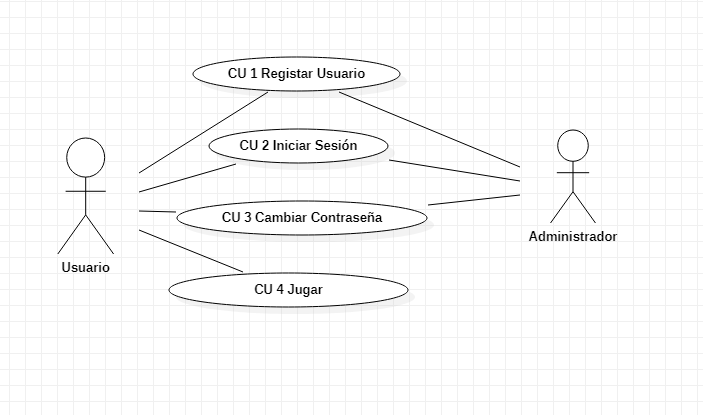
\includegraphics[scale=0.7]{imgs/CasosDeUso}
    \caption{Diagrama de Casos de Uso}
\end{figure}
\subsubsection{Tabla descriptiva de Caso de Uso 1}
\begin{tabular}{|M{5cm}|c|}
\hline
Caso de Uso & CU1 Registrar Usuario\\ \hline
Versión & 1.1\\ \hline
Autor(es) & Itzcoatl Rodrigo Pineda Vieyra\\ \hline
Revisor & Izaird Alexander Mothelet Delgado \\ \hline
Actor(es) & Usuario Final \\ \hline
Entradas & correo electrónico, contraseña, \\ & Cuenta de Google \\ \hline
Salidas & Cuenta de usuario creada \\ \hline
Pre-condiciones & Instalar y abrir la aplicación \\ \hline
Post-condiciones & Cuenta de usuario creada\\ \hline
Mensajes & MSN1: "Ingrese un texto válido"\\
		 & MSN2: "Bienvenido"\\ \hline
Fuente & RF1,RF3 \\ \hline	
	Trayectoria & Trayectoria A (principal)\\
		& 1.   El usuario seleccionará la opción de registrarse.\\
		& 2.   Se ingresarán los datos correspondientes.\\
		& 3.   Se creará correctamente la cuenta del usuario\\
		& 4.   Se envia un correo de confirmación al email proporcionado \\	
	& Trayectoria B\\
	& 1.   El usuario seleccionará la opción de registrarse.\\
	& 2.   Se proporcionará una cuenta de Google\\
	& 3.   Se confirma y se dan los permisos correspondientes.\\
	& 4   Se creará correctamente la cuenta del usuario.\\ \hline
\end{tabular}
\subsubsection{Tabla descriptiva de Caso de Uso 2}
\begin{tabular}{|M{5cm}|c|}
\hline
Caso de Uso & CU2 Iniciar Sesión\\ \hline
Versión & 1.1\\ \hline
Autor(es) & Itzcoatl Rodrigo Pineda Vieyra\\ \hline
Revisor & Izaird Alexander Mothelet Delgado \\ \hline
Actor(es) & Usuario Final \\ & Administrador\\ \hline
Entradas &  Correo electrónico, contraseña\\ & Cuenta de Google \\ \hline
Salidas & Sesión de usuario \\ \hline
Pre-condiciones & Instalar y abrir la aplicación \\ \hline
Post-condiciones & Sesión iniciada\\ \hline
Mensajes & MSN1: "Ingrese un texto válido"\\
		   & MSN2: "Bienvenido"\\ \hline
Fuente & RF2,RF3 \\ \hline	
	Trayectoria & Trayectoria A (principal)\\
		& 1.   El usuario ingresa sus credenciales (correo y contraseña).\\
		& 2.   Se valida si existen coincidencias de las credenciales proporcionadas\\
		& 3. Se inicia sesión o se despliega un mensaje de error.\\
	& Trayectoria B\\
	& 1.   El usuario seleccionará la opción de registrarse.\\
	& 2.   Se proporcionará una cuenta de Google\\
	& 3.   Se inicia sesión.\\ \hline
\end{tabular}
\subsubsection{Tabla descriptiva de Caso de Uso 3}
\begin{tabular}{|M{5cm}|c|}
\hline
Caso de Uso & CU3 Cambiar Contraseña\\ \hline
Versión & 1.1\\ \hline
Autor(es) & Itzcoatl Rodrigo Pineda Vieyra\\ \hline
Revisor & Izaird Alexander Mothelet Delgado \\ \hline
Actor(es) & Usuario Final \\ \hline
Entradas &  Correo y contraseña nueva \\ \hline
Salidas & Cuenta con ccontraeña nueva \\ \hline
Pre-condiciones & Iniciar Sesión \\ \hline
Post-condiciones & \\ \hline
Mensajes & MSN1: "Se envio el correo para reestablecer contraseña"\\
		   & MSN2: "Bienvenido"\\ \hline
Fuente & RF4 \\ \hline	
	Trayectoria
		& 1.	El usuario selecciona el Modo Infinito del menu lateral\\
		& 2.    El usuario responde  las preguntas \\
		& 3.	El usuario comete 3 errores o presiona el boton de regreso, terminando el juego.\\ \hline
\end{tabular}
\subsubsection{Tabla descriptiva de Caso de Uso 4}
\begin{tabular}{|M{5cm}|c|}
\hline
Caso de Uso & CU4 Jugar\\ \hline
Versión & 1.1\\ \hline
Autor(es) & Itzcoatl Rodrigo Pineda Vieyra\\ \hline
Revisor & Izaird Alexander Mothelet Delgado \\ \hline
Actor(es) & Usuario Final \\ \hline
Entradas &  Respuesta, modo de juego, operación, dificultad \\ \hline
Salidas & Puntuación \\ \hline
Pre-condiciones & Iniciar Sesión \\ \hline
Post-condiciones & Puntuación\\ \hline
Mensajes & \\
Fuente & RF4, RF5 \\ \hline	
	Trayectoria
		& 1.	El usuario selecciona Juegos del menu lateral o de la pantalla principal\\
		& 2. El usuario selecciona el modo de juego, el tipo de operaciones y la dificultad.\\
		& 3.    El usuario responde  las preguntas \\
		& 4.	Al completar la ronda de preguntas o cometer 3 errores en caaso del modo infinito, termina el juego.\\ 
		& 5. 	Se informa al usuario de su puntuación y se registra en el leaberboard\\ \hline
\end{tabular}
\subsubsection{Tabla descriptiva de Caso de Uso 5}
\begin{tabular}{|M{5cm}|c|}
\hline
Caso de Uso & CU5 Consultar Leaderboard\\ \hline
Versión & 1.1\\ \hline
Autor(es) & Itzcoatl Rodrigo Pineda Vieyra\\ \hline
Revisor & Izaird Alexander Mothelet Delgado \\ \hline
Actor(es) & Usuario Final \\ \hline
Entradas &  Modo de juego, operacion \\ \hline
Salidas & Leaderboard \\ \hline
Pre-condiciones & Iniciar Sesión\\ \hline
Post-condiciones & \\ \hline
Mensajes & \\
Fuente &  \\ \hline	
	Trayectoria
		& 1.	El usuario selecciona Leaderboards del menu lateral o de la pantalla principal \\
		& 2. El usuario selecciona el modo de juego, el tipo de operaciones.\\
		& 3.    El usuario responde  las preguntas \\
		& 4.	Se despliega el leaderboard correspondiente\\ \hline
\end{tabular}
\subsubsection{Tabla descriptiva de Caso de Uso 6}
\begin{tabular}{|M{5cm}|c|}
\hline
Caso de Uso & CU6 Consultar Logros\\ \hline
Versión & 1.1\\ \hline
Autor(es) & Itzcoatl Rodrigo Pineda Vieyra\\ \hline
Revisor & Izaird Alexander Mothelet Delgado \\ \hline
Actor(es) & Usuario Final \\ \hline
Entradas &  Modo de juego, operacion \\ \hline
Salidas & Leaderboard \\ \hline
Pre-condiciones & Iniciar Sesión,  \\ \hline
Post-condiciones & \\ \hline
Mensajes & \\
Fuente &  \\ \hline	
	Trayectoria
		& 1. El usuario selecciona Logros del menu lateral o de la pantalla principal \\
		& 2. Se despliega la lista de logros \\ \hline
\end{tabular}
\subsubsection{Tabla descriptiva de Caso de Uso 7}
\begin{tabular}{|M{5cm}|c|}
\hline
Caso de Uso & CU7 Subir Plantilla\\ \hline
Versión & 1.1\\ \hline
Autor(es) & Izaird Alexander Mothelet Delgado\\ \hline
Revisor &  Itzcoatl Rodrigo Pineda Vieyra \\ \hline
Actor(es) & Administrador \\ \hline
Entradas &  Plantilla, valores \\ \hline
Salidas & Leaderboard \\ \hline
Pre-condiciones & Iniciar Sesión \\ \hline
Post-condiciones & Plantilla en Base de Datos\\ \hline
Mensajes & \\
Fuente &  \\ \hline	
	Trayectoria
		& 1. El administrador selecciona Plantillas del menu lateral o de la pantalla principal \\
		& 2. Se despliega la lista de plantillas\\ 
		& 3. Se presiona el botón de + para agregar plantilla\\
		& 4. Se rellenan los campos de plantilla y valores respecctivos a  cada dificultad \\		
		\hline
		
\end{tabular}
\subsubsection{Tabla descriptiva de Caso de Uso 8}
\begin{tabular}{|M{5cm}|c|}
\hline
Caso de Uso & CU7 Otorgar permisos\\ \hline
Versión & 1.1\\ \hline
Autor(es) & Itzcoatl Rodrigo Pineda Vieyra \\ \hline
Revisor &  Izaird Alexander Mothelet Delgado \\ \hline
Actor(es) & Administrador \\ \hline
Entradas &  Plantilla, valores \\ \hline
Salidas & 1 \\ \hline
Pre-condiciones & Iniciar Sesión  \\ \hline
Post-condiciones & Usuario con permisos de adminitrador\\ \hline
Mensajes & \\
Fuente &  \\ \hline	
	Trayectoria
		& 1. El administrador selecciona Usuarios del menu lateral o de la pantalla principal \\
		& 2. Se despliega la lista de usuarios\\ 
		& 3. Se selecciona el usuario al que se desea otorgar o revocar permisos \\
		& 4. Se checa la checkbox para otorgar permisos\\
		& 5. Se selecciona la paloma para confirmar\\		
		\hline
\end{tabular}
\subsection{Análisis de Interfaces}
%Descripcion de tipo de interfaz y por que
Las interfaces deberán ser optimizadas para dispositivos móviles. Deberá considerarse la capacidad touch de dichos dispositivos. La primera pantalla será para Iniciar sesión por medio del correo y contraseña junto con un botón para registrarse. La pantalla de registro solicitará el correo, contraseña y confirmación de la contraseña. Se deberá contar con botones para acceder al perfil de usuario, leaderboards y logros en una barra de navegación, esta puede ser horizontal o vertical. La pantalla de ejercicios mostrará la puntuación en todo momento en una esquina y el número de respuestas correctas consecutivas junto un icono. En caso de haber tiempo para responder a una pregunta habrá una barra horizontal en la parte superior la cual irá desapareciendo conforme transcura el tiempo asignado al usuario para dar respuesta a la pregunta, la cual irá  desaapareciendo de derecha a izquierda.
\subsection{Análisis de la Base de Datos}%Narrativa
Para desarrollar esta aplicación se cuenta con una entidad Usuario con campos correo (llave primaria) y contraseña, con el correo como identificador de la entidad, pues no se permiten correos duplicados. Los Logros y leaderboards son manejaados por el servicio externo de Google Play Juegos por lo cual no se incluyen en nuestra base de datos
\subsection{Tecnologías usadas}
\pagebreak
\section{Diseño}
\subsection{Arquitectura general del sistema}%Imagen arquitectura y descripcion%Imagen arquitectura y descripcion
La arquitectura se compone de 4 subsistemas (ver figura 2).  El primer subsistema es el de Registro e inicio de sesión y es el encargado de dar de alta y permitir el acceso a los usuarios ya registrados. El segundo subsistema corresponde a los módulos que interactuan con el usuario, estos son el módulo de ejercicios, encargado de proporcionar ejercicios al usuario, y el módulo evaluador de logros y mecánicas, el cual se encarga de llevar el registro de la puntuación, logros y niveles. El Subsistema de administardor incluye los módulos generador de problemas y evaluador de expresiones, los cuales se usan para generar los ejercicios para el usuario. También se incluye un módulo de actualización y consulta de dichos ejercicios. El último subsistema es el de estadísticas y progreso, el cual lleva el registro de los logros globales del usuario.  
\begin{figure}[H]
    \centering
    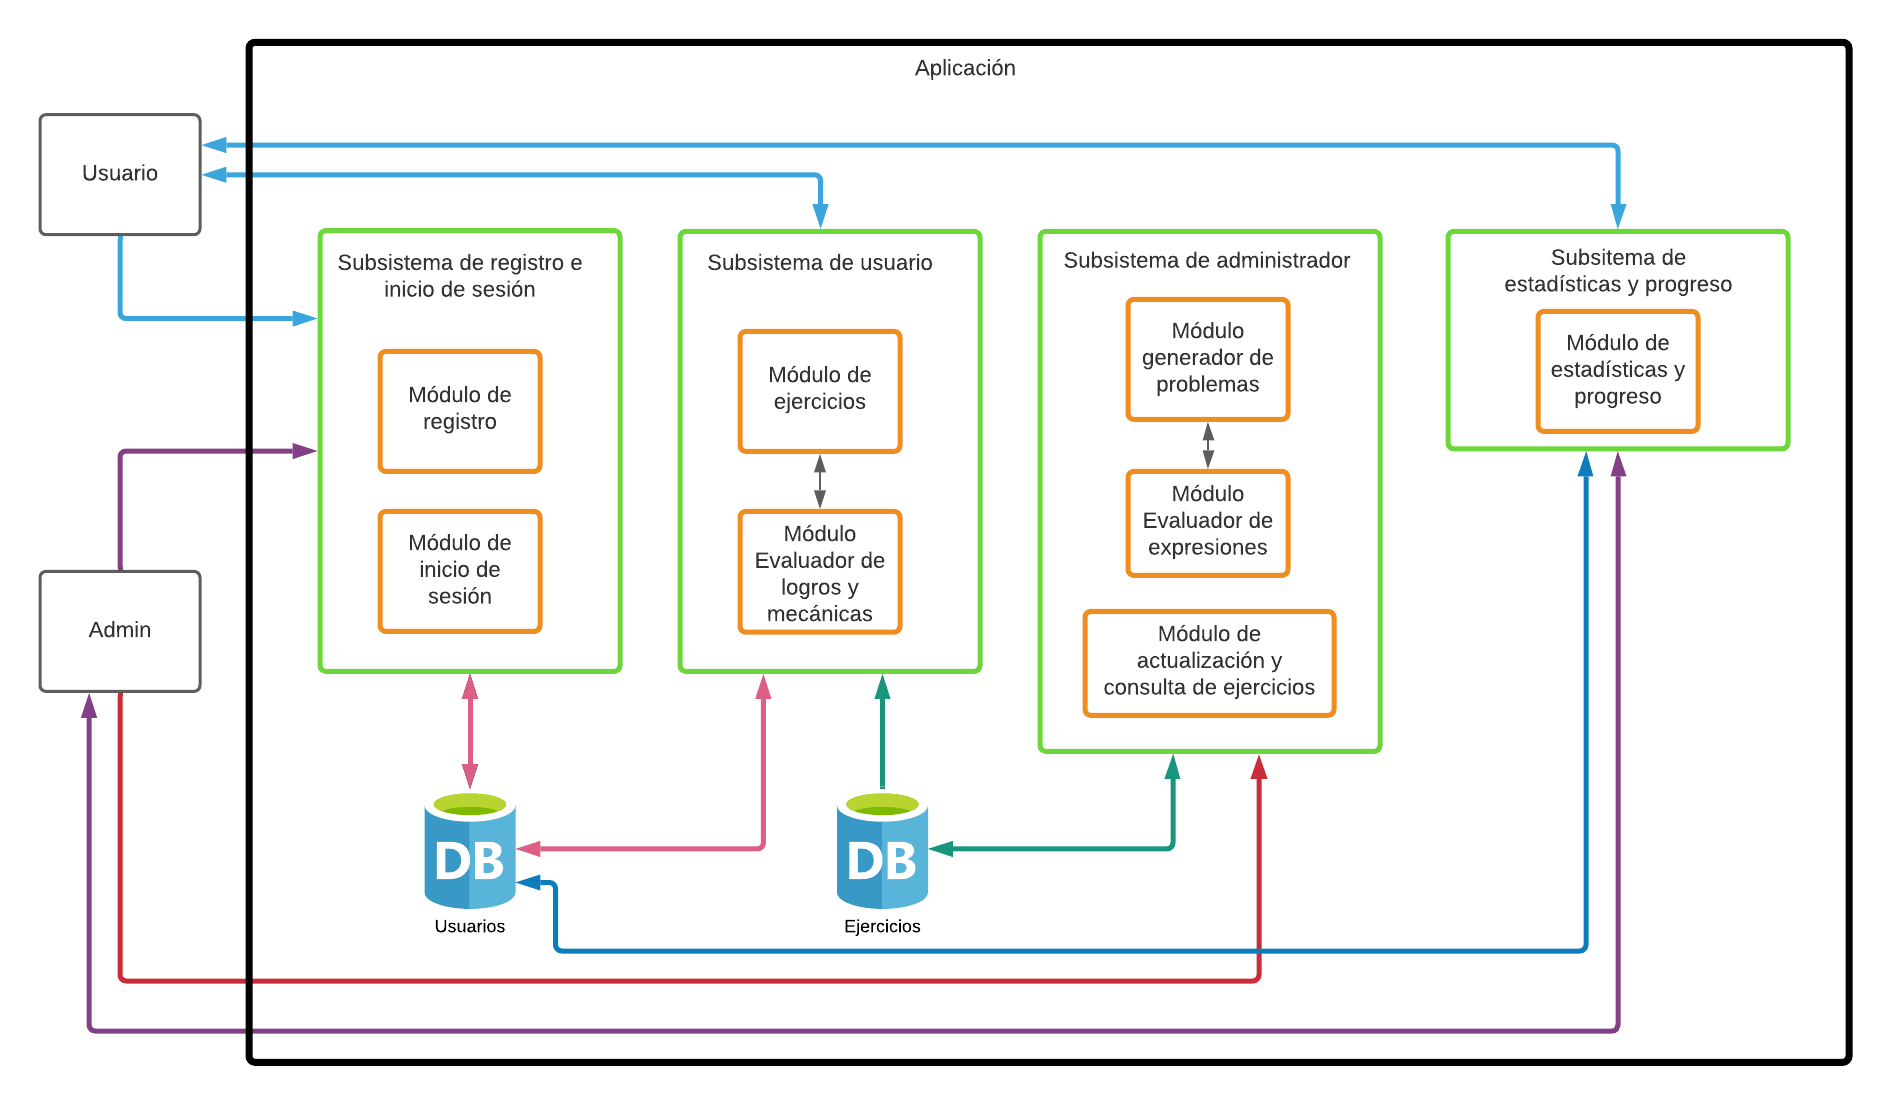
\includegraphics[scale=0.65]{imgs/Arquitectura}
    \caption{Arquitectura}
\end{figure}

\subsection{Diseño de Base de Datos}%diagrama entidad relacion pk subrayada
\begin{figure}[H]
    \centering
    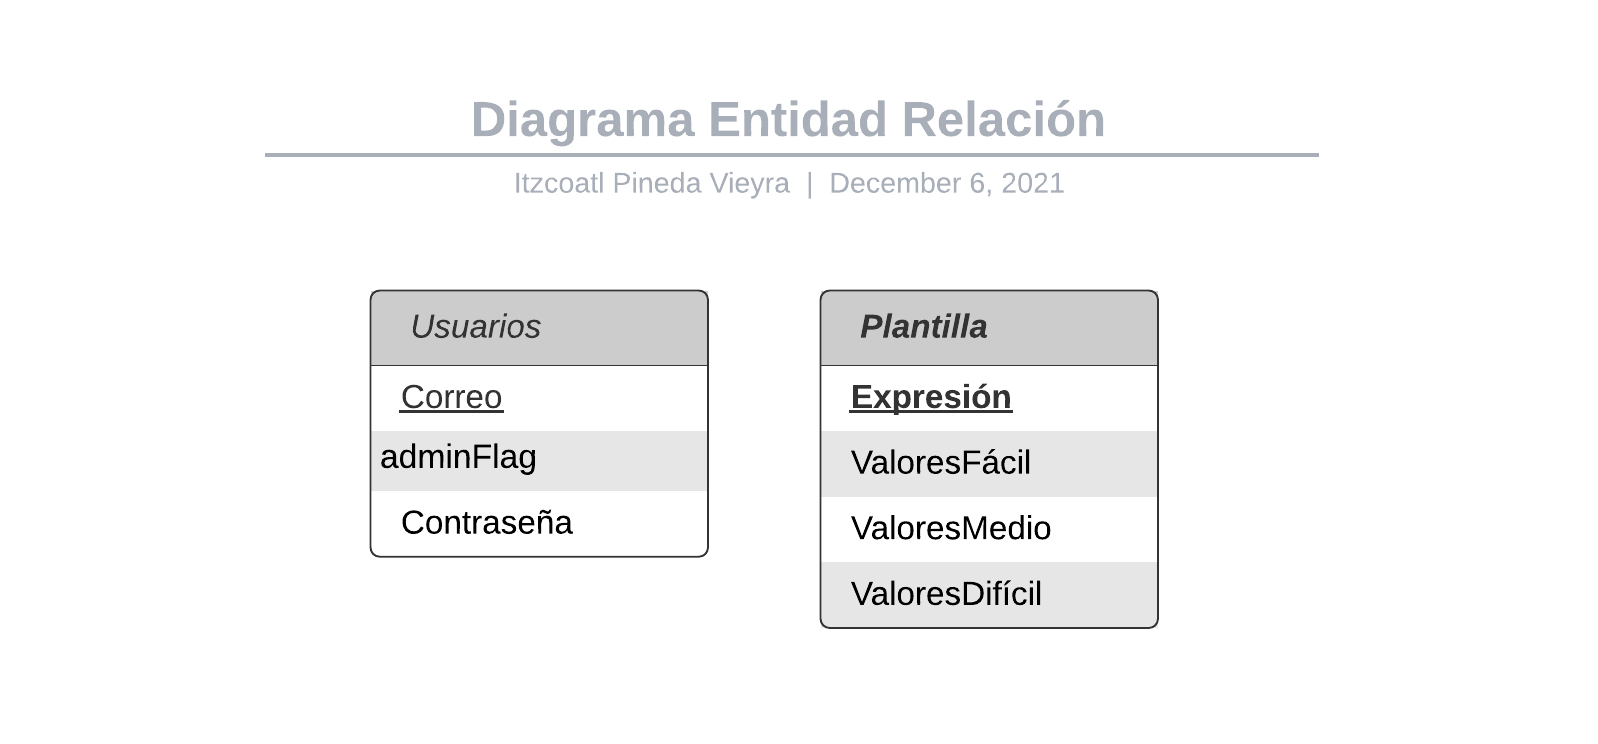
\includegraphics[scale=0.9]{imgs/BSD}
    \caption{Diagrama entidad relación}
\end{figure}
\subsection{Diseño de Interfaces}%mock-ups
En este apartado se presentarán los diseños de las interfaces previamente descritras.
\pagebreak
\begin{figure}[H]
    \centering
    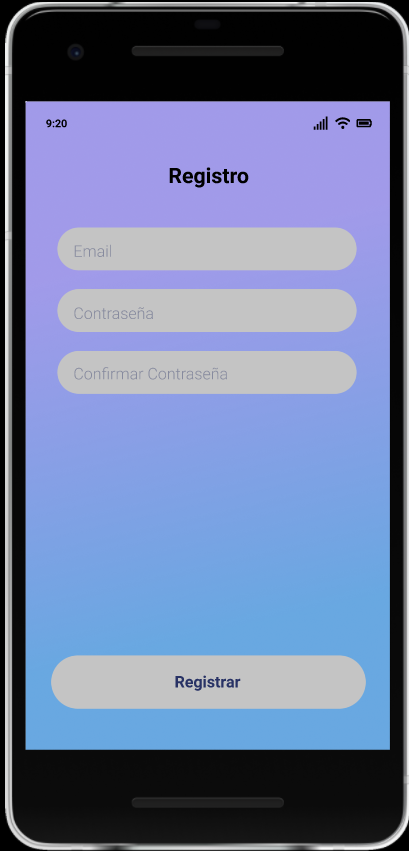
\includegraphics[scale=0.9]{imgs/Figma/Registro2} 
    \caption{Registro}
\end{figure}
\begin{figure}[H]
    \centering
    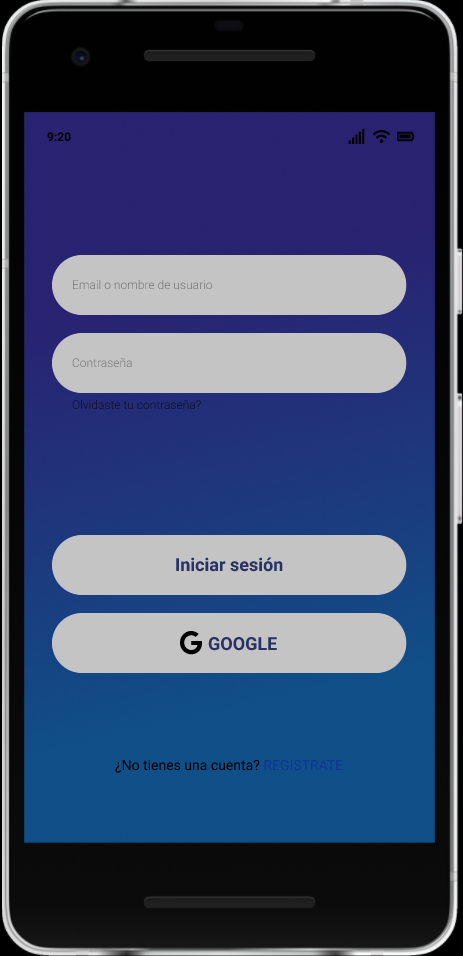
\includegraphics[scale=0.9]{imgs/Figma/Login}
    \caption{Login}
\end{figure}
\begin{figure}[H]
    \centering
    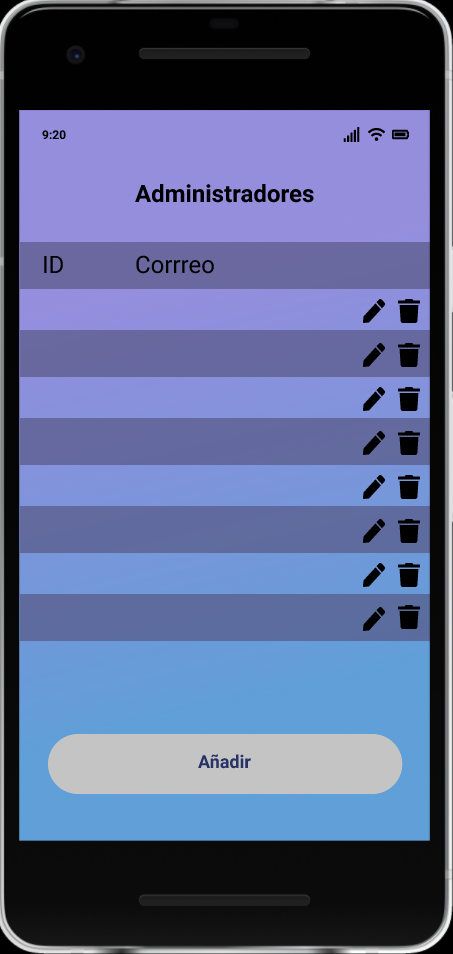
\includegraphics[scale=0.9]{imgs/Figma/Admins}
    \caption{Administrador}
\end{figure}
\begin{figure}[H]
    \centering
    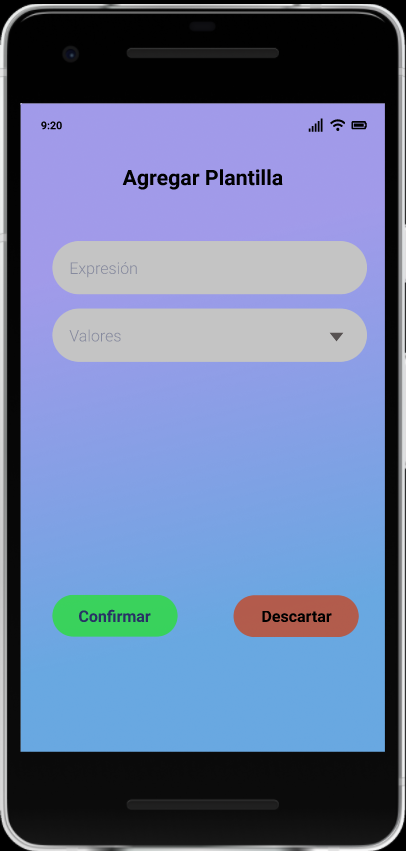
\includegraphics[scale=0.9]{imgs/Figma/Plantilla}
    \caption{Plantillas}
\end{figure}
\begin{figure}[H]
    \centering
    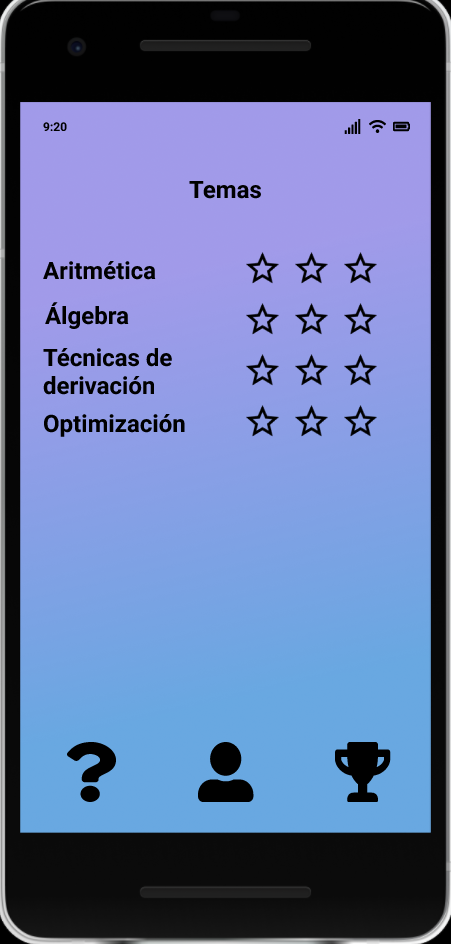
\includegraphics[scale=0.9]{imgs/Figma/Temas}
    \caption{Selección de tema}
\end{figure}
\begin{figure}[H]
    \centering
    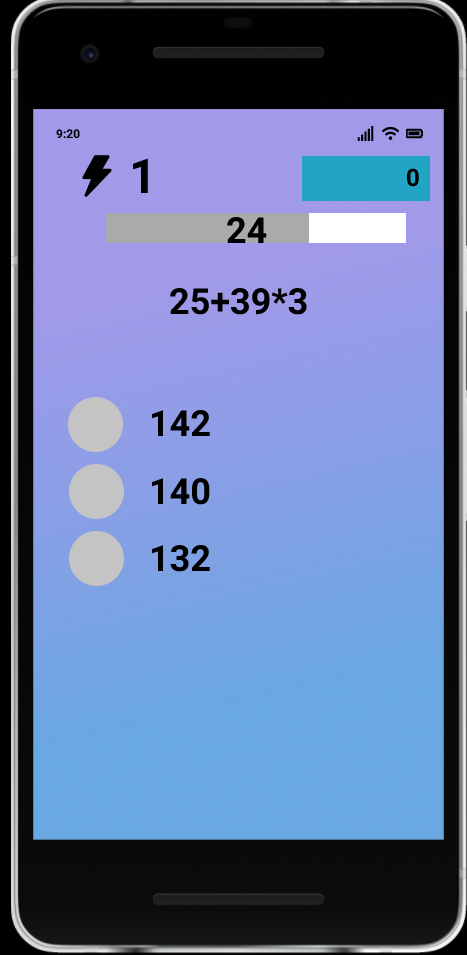
\includegraphics[scale=0.9]{imgs/Figma/Ejemplo}
    \caption{Ejemplo}
\end{figure}
\begin{figure}[H]
    \centering
    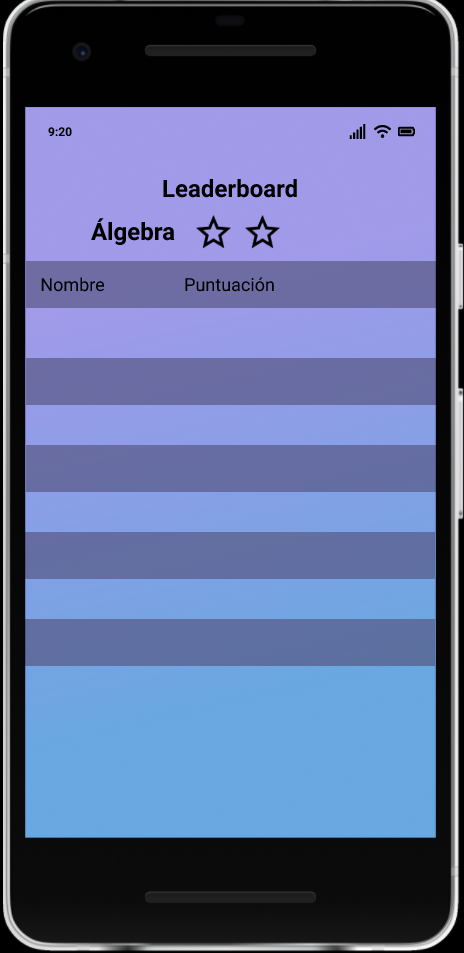
\includegraphics[scale=0.9]{imgs/Figma/Leaderboard}
    \caption{Leaderboard}
\end{figure}

\subsection{Metodología}
La metodología que se ha elegido para el desarrollo de este proyecto es Feature planninig 
\cite{hunt2006feature}, también conocida como Feature Driven 
Development F.D.D Esta metodología iterativa orientada a objetos, consistente en planear 
la estructura general del proyecto, realizar una lista de características, planear y finalmente 
construir cada una de ellas. En nuestro caso podemos ver cada característica como un tema y ciertas 
funcionalidades adicionales que deseamos integrar. Para garantizar la variedad de ejercicios se 
pretende usar técnicas de generación por procedimientos.

La lista de características sería la siguiente:
\begin{enumerate}
	\item Sistema de puntuación.
	\item Ejercicios de Aritmética.
	\begin{enumerate}
		\item Adición y sustracción.
		\item multiplicación.
		\item División.
	\end{enumerate}
	\item Evaluador de expresiones.
	\item Niveles de dificultades.
	\item Leaderboards.
	\item Títulos, Iconos para desbloquear con puntos.
	\item Estadísticas del jugador.
\end{enumerate}
\pagebreak
\section{Implementación}
%Subsistema de registro e ingreso Captura de pantalla con descripcion citar mock up de la pantalla
El subsistema de registro e ingreso fue implementado con Firebase 
\begin{figure}[H]
    \centering
    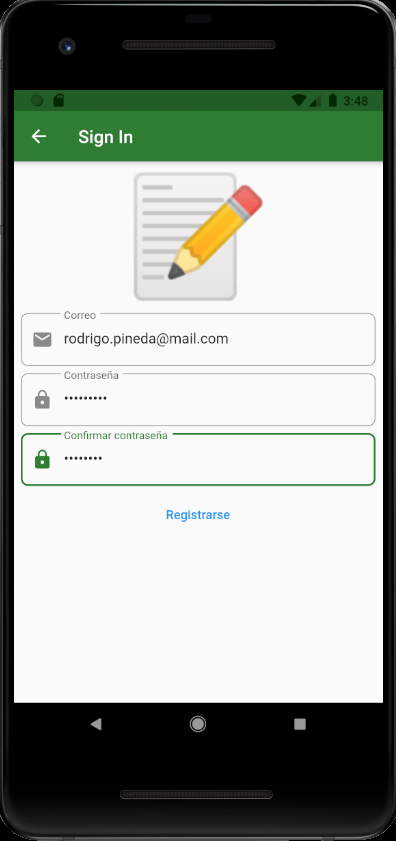
\includegraphics[scale=0.8]{imgs/Imp/Registro}
    \caption{Implementación Registro}
\end{figure}
\begin{figure}[H]
    \centering
    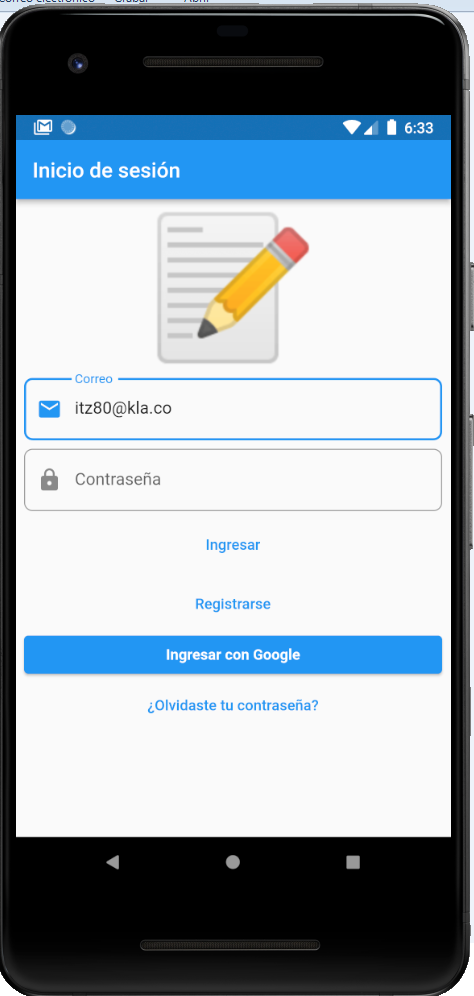
\includegraphics[scale=0.8]{imgs/Imp/Login1}
    \caption{Implementación de Login}
\end{figure}
\begin{figure}[H]
    \centering
    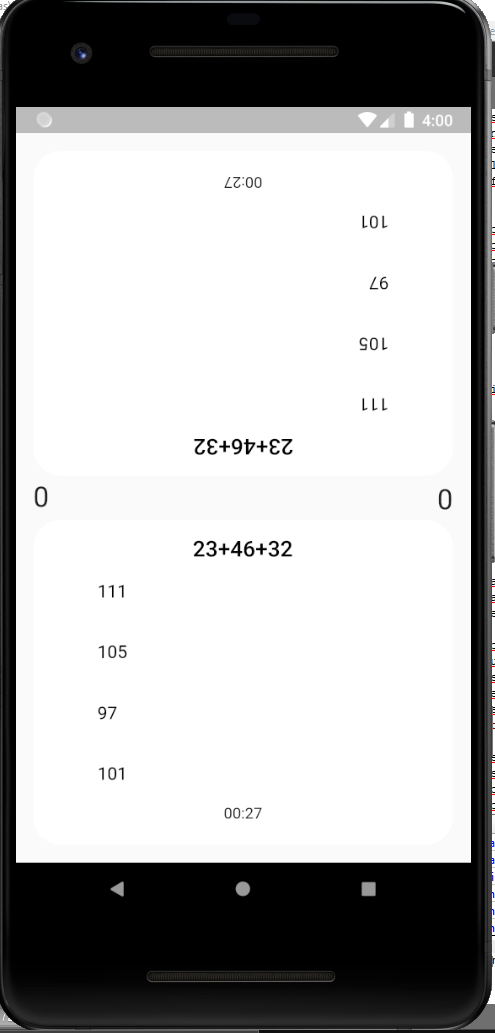
\includegraphics[scale=0.8]{imgs/Imp/Pvp}
    \caption{Implementación de modo jugador contra jugador}
\end{figure}
\begin{figure}[H]
    \centering
    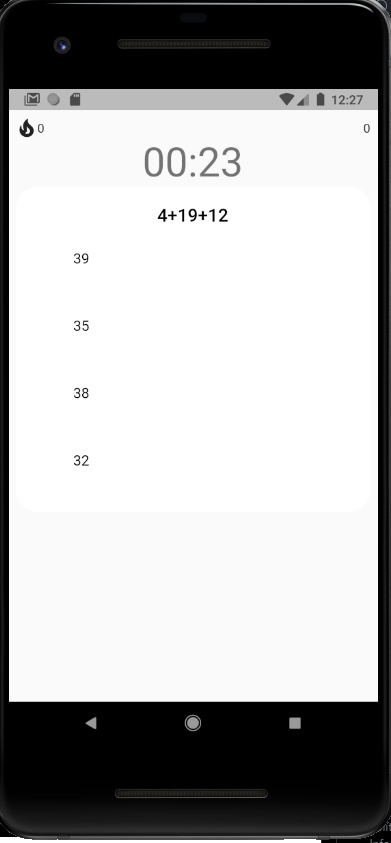
\includegraphics[scale=0.8]{imgs/Imp/Endless}
    \caption{Implementación de modo infinito}
\end{figure}
\begin{figure}[H]
    \centering
    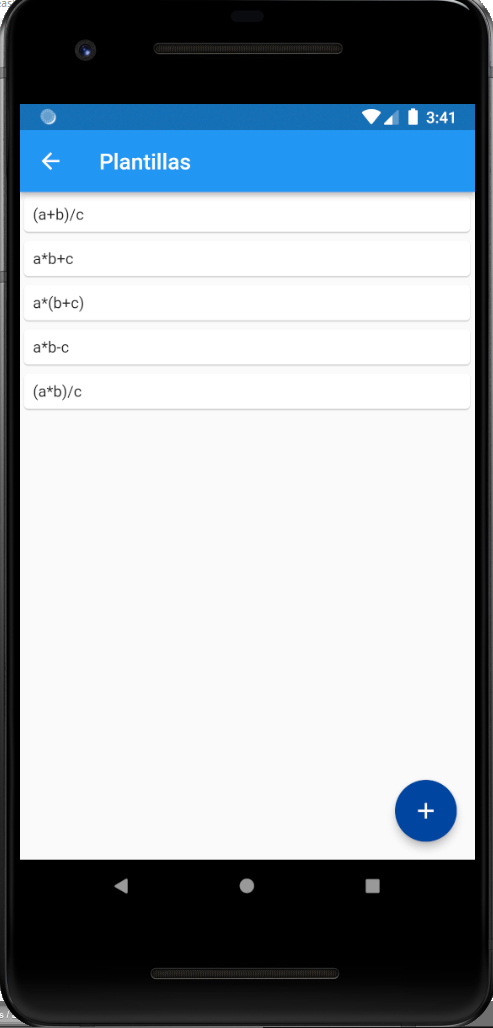
\includegraphics[scale=0.8]{imgs/Imp/Plantillas}
    \caption{Implementación de Plantillas}
\end{figure}
\begin{figure}[H]
    \centering
    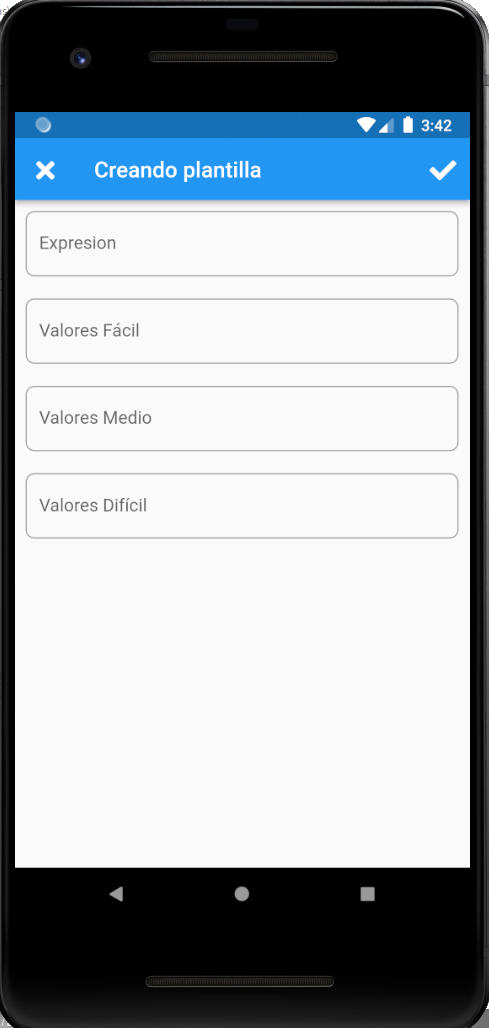
\includegraphics[scale=0.8]{imgs/Imp/Plantillas2}
    \caption{Implementación de Plantillas}
\end{figure}
\begin{figure}[H]
    \centering
    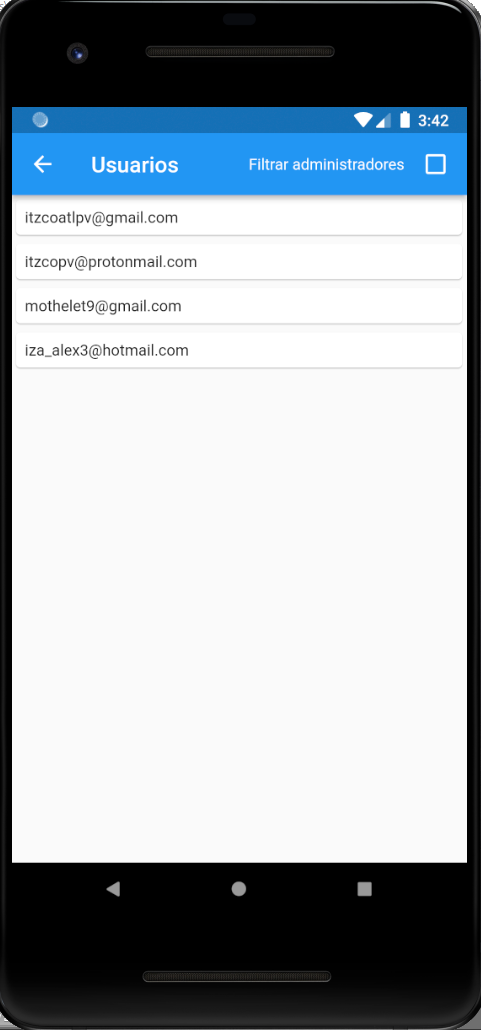
\includegraphics[scale=0.8]{imgs/Imp/Usuarios}
    \caption{Implementación de Usuarios}
\end{figure}
\section{Pruebas}%Que pruebas se le hicieron al sistema
Se validó el correo con una expresión regular. Algunos ejemplos de correos validos
\begin{itemize}
	\item itz80@kla.co
	\item \verb |itz!&*%^7@protonmail.net|
	\item 1A!e@protonmail.com
\end{itemize}

\pagebreak
\printbibliography


\end{document}